% This work is made available under the terms of the
% Creative Commons Attribution-ShareAlike 4.0 license,
% http://creativecommons.org/licenses/by-sa/4.0/.
%
% Version: $Revision$

\documentclass[a4paper]{book}

\usepackage{wrapfig}
\usepackage{graphicx}
\usepackage{hyperref}
\usepackage{multirow}
\usepackage{scalefnt}
\usepackage{tikz}

% watermark -- for draft stage
\usepackage[firstpage]{draftwatermark}
\SetWatermarkLightness{0.9}
\SetWatermarkScale{5}

% Copyright (c) 2009 by the University of Waikato, Hamilton, NZ. 
% This work is made available under the terms of the 
% Creative Commons Attribution-ShareAlike 3.0 license, 
% http://creativecommons.org/licenses/by-sa/3.0/. 
%
% Version: $Revision$

\newenvironment{tight_itemize}{
\begin{itemize}
  \setlength{\itemsep}{1pt}
  \setlength{\parskip}{0pt}
  \setlength{\parsep}{0pt}}{\end{itemize}
}

\newenvironment{tight_enumerate}{
\begin{enumerate}
  \setlength{\itemsep}{1pt}
  \setlength{\parskip}{0pt}
  \setlength{\parsep}{0pt}}{\end{enumerate}
}

% if you just need a simple heading
% Usage:
%   \heading{the text of the heading}
\newcommand{\heading}[1]{
  \vspace{0.3cm} \noindent \textbf{#1} \newline
}

\newcommand{\icon}[1]{\tikz[baseline=-3pt]\node[inner sep=0pt,outer sep=0pt]{\includegraphics[height=1.1em]{#1}};}


\title{
  \textbf{ADAMS} \\
  {\Large \textbf{A}dvanced \textbf{D}ata mining \textbf{A}nd \textbf{M}achine
  learning \textbf{S}ystem} \\
  {\Large Module: adams-visualstats} \\
  \vspace{1cm}
  
\includegraphics[width=2cm]{images/visualstats-module.png} \\
}
\author{
  Peter Reutemann
}

\setcounter{secnumdepth}{3}
\setcounter{tocdepth}{3}

\begin{document}

\begin{titlepage}
\maketitle

\thispagestyle{empty}
\center
\begin{table}[b]
	\begin{tabular}{c l l}
		\parbox[c][2cm]{2cm}{\copyright 2012-2016} &
		\parbox[c][2cm]{5cm}{
\includegraphics[width=5cm]{images/coat_of_arms.pdf}} \\
	\end{tabular}
	
\includegraphics[width=12cm]{images/cc.png} \\
\end{table}

\end{titlepage}

\tableofcontents
\listoffigures
%\listoftables

%%%%%%%%%%%%%%%%%%%%%%%%%%%%%%%%%%%
\chapter{Introduction}
Visualizing data is very important to understand the data that you are dealing
with. Even more important it is to visualize the statistics and evaluations 
that you generated in order to better understand your models, whether they are
working properly and not just plain useless. The \textit{visualstats} module
contains some useful visualizations for statistics which are discussed in the 
next chapter.

%%%%%%%%%%%%%%%%%%%%%%%%%%%%%%%%%%%
\chapter{Flow}
\section{Actors}
The following transformers are available:
\begin{tight_itemize}
	\item \textit{ControlChart} -- computes control chart statistics from the
	incoming data.
\end{tight_itemize}
The following sinks are available:
\begin{tight_itemize}
	\item \textit{BoxPlot} -- displays box plots \cite{boxplot} of the attributes
	of a dataset.
	\item \textit{ControlChartPlot} -- displays control chart data.
	\item \textit{FourInOneDisplay} -- Plots the residuals\cite{4in1} in various ways:
	probability plot, fit, histogram \cite{histogram}, order.
	\item \textit{Histogram} -- plots a histogram\cite{histogram} of numeric data.
	\item \textit{MatrixPlot} -- scatter plots of attributes, all vs all.
	\item \textit{ProbabilityPlotDisplay} -- plots the probabilities of 
	predictions, with option regression line, e.g., a normal probability
	plot \cite{normalprobplot}.
	\item \textit{ScatterDisplay} -- plots one attribute vs another 
	\cite{scatterplot}.
	\item \textit{ZScoreDisplay} -- displays the z-scores of predictions.
\end{tight_itemize}

\newpage
\section{Examples}
The following sections demonstrate how to use the previously introduced actors.

\subsection{Box plot}
The \textit{BoxPlot}\footnote{adams-visualstats-box\_plots.flow} sink takes
a WEKA dataset (\texttt{weka.core.Instances}) object as input. You can specify
the range of attributes to display.

The plot, as it shows the range for an attribute, makes only sense to use for
numeric attributes. Hence it is easiest to use a filter to remove non-numeric
attributes, e.g., \textit{RemoveType} with \textit{numeric} attributes as the
type to remove and the \textit{invertSelection} flag 
enabled\footnote{adams-visualstats-box\_plots.flow}.

\begin{figure}[ht]
  \begin{minipage}[t]{0.5\linewidth}
    \centering
    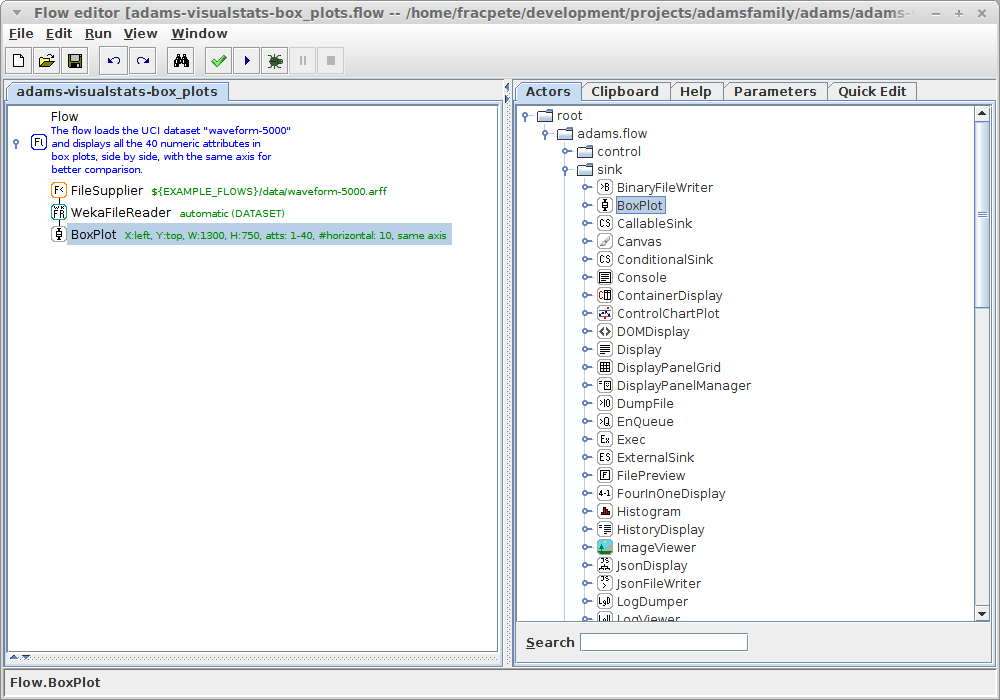
\includegraphics[width=5.5cm]{images/boxplot-flow.png}
    \caption{Box plot flow.}
    \label{boxplot-flow}
  \end{minipage}
  \hspace{0.5cm}
  \begin{minipage}[t]{0.5\linewidth}
    \centering
    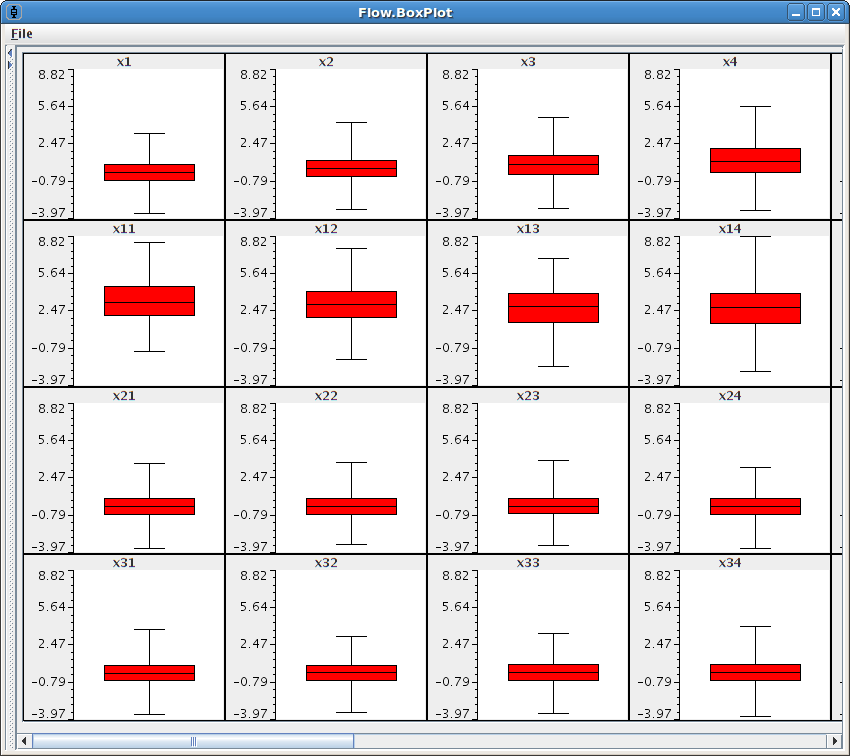
\includegraphics[width=6.0cm]{images/boxplot-output.png}
    \caption{Box plot output.}
    \label{boxplot-output}
  \end{minipage}
\end{figure}

\clearpage
\subsection{Histogram}
With the \textit{Histogram} sink, you can quickly plot an attribute of
a WEKA dataset or any double array. Figures \ref{histogram-flow} and 
\ref{histogram-output} show a flow\footnote{adams-visualstats-histogram.flow}
that generates a histogram for the \textit{sepallength} attribute of the
UCI dataset \textit{iris}.

\begin{figure}[ht]
  \begin{minipage}[t]{0.5\linewidth}
    \centering
    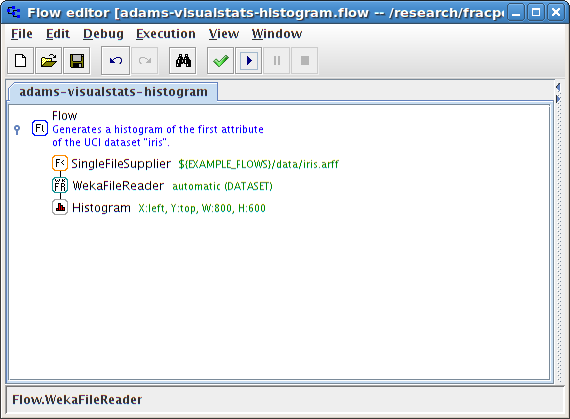
\includegraphics[width=5.5cm]{images/histogram-flow.png}
    \caption{Histogram flow.}
    \label{histogram-flow}
  \end{minipage}
  \hspace{0.5cm}
  \begin{minipage}[t]{0.5\linewidth}
    \centering
    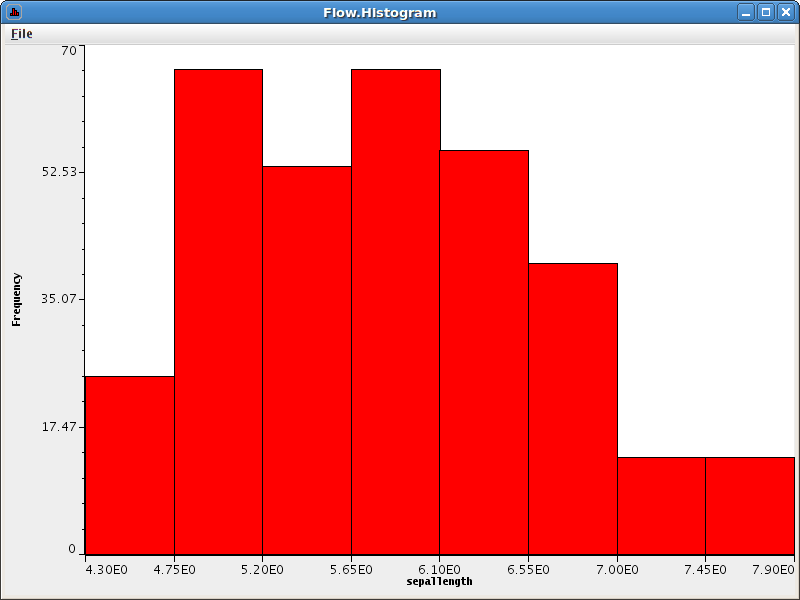
\includegraphics[width=6.0cm]{images/histogram-output.png}
    \caption{Histogram output.}
    \label{histogram-output}
  \end{minipage}
\end{figure}

\clearpage
\subsection{4-in-1}
The 4-in-1 plot is a quick solution to plotting the residuals from a regression 
analysis\cite{regression} in a single plot. The four displays are:
\begin{tight_itemize}
	\item \textit{normal probability plot} -- if the data points are along
	the diagonal, the data seems to be normal distributed. An s-shape suggests
	a uniform distribution.
	\item \textit{histogram} -- a bell-shaped histogram indicates a normal
	distribution.
	\item \textit{versus fit} -- plots the residuals against their predicted
	value, with a random distribution around the mean indicating a good fit
	of the model.
	\item \textit{versus order} -- shows the residuals how the were generated
	by the model, one after the other. A \textit{trumpet} shape here indicates
	a non-constant variance.
\end{tight_itemize}
Figure \ref{4in1-flow} shows a flow for generating a 4-in-1 plot based on a
cross-validation run of LinearRegression on the UCI dataset \textit{bodyfat}.
In Figure \ref{4in1-output} you can see the generated plot.

\begin{figure}[ht]
  \begin{minipage}[t]{0.5\linewidth}
    \centering
    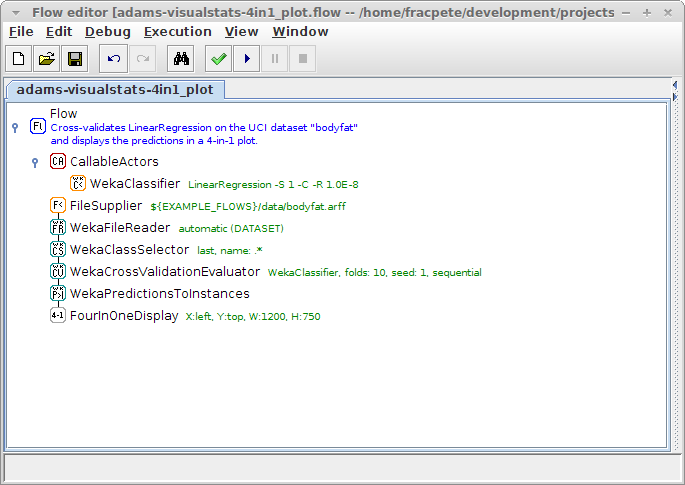
\includegraphics[width=5.5cm]{images/4in1-flow.png}
    \caption{Flow using 4-in-1 display.}
    \label{4in1-flow}
  \end{minipage}
  \hspace{0.5cm}
  \begin{minipage}[t]{0.5\linewidth}
    \centering
    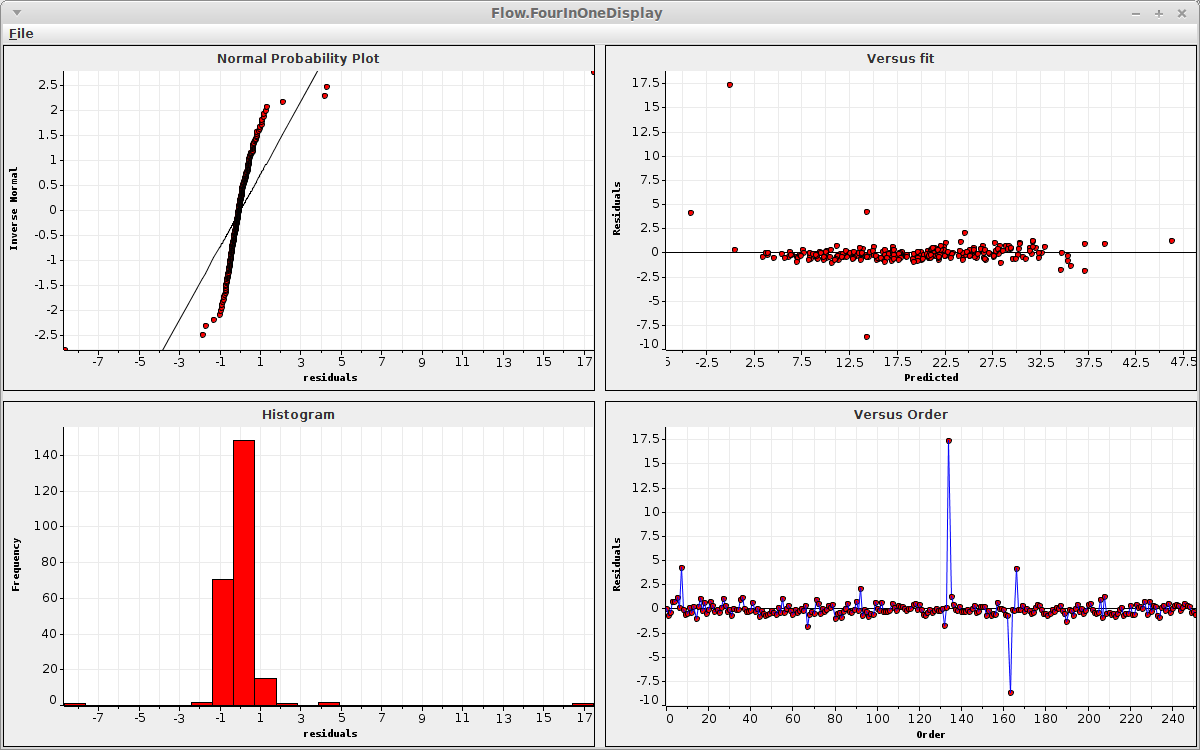
\includegraphics[width=6.0cm]{images/4in1-output.png}
    \caption{4-in-1 display output.}
    \label{4in1-output}
  \end{minipage}
\end{figure}

\noindent ADAMS comes with some example flows using different 
datasets.\footnote{adams-visualstats-4in1\_plot.flow}
\footnote{adams-visualstats-4in1\_plot2-slug\_original.flow}
\footnote{adams-visualstats-4in1\_plot2-slug\_ln.flow}

\clearpage
\subsection{Matrix plot}
The \textit{MatrixPlot} sink simply plots all attributes versus each other.
This, in combination with overlays such as LOWESS (locally weighted 
scatterplot smoothing), allows you to determine whether there is a relationship
(or collinearity) between attributes. Figures \ref{matrixplot-flow} shows a 
flow\footnote{adams-visualstats-matrix\_plot.flow} that displays the UCI dataset
\textit{iris} as a matrix plot (\ref{matrixplot-output}). The almost straight 
line of the LOWESS overlay shows, that there is a linear relationship 
between \textit{petallength} and \textit{petalwidth}. The nominal class also
has a good separation for the \textit{petallength} and \textit{petalwidth}
attributes (see bottom row).

\begin{figure}[ht]
  \begin{minipage}[t]{0.5\linewidth}
    \centering
    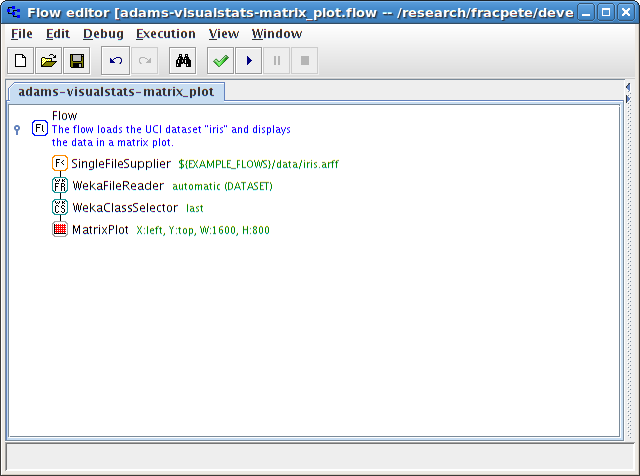
\includegraphics[width=5.5cm]{images/matrixplot-flow.png}
    \caption{Matrix plot flow.}
    \label{matrixplot-flow}
  \end{minipage}
  \hspace{0.5cm}
  \begin{minipage}[t]{0.5\linewidth}
    \centering
    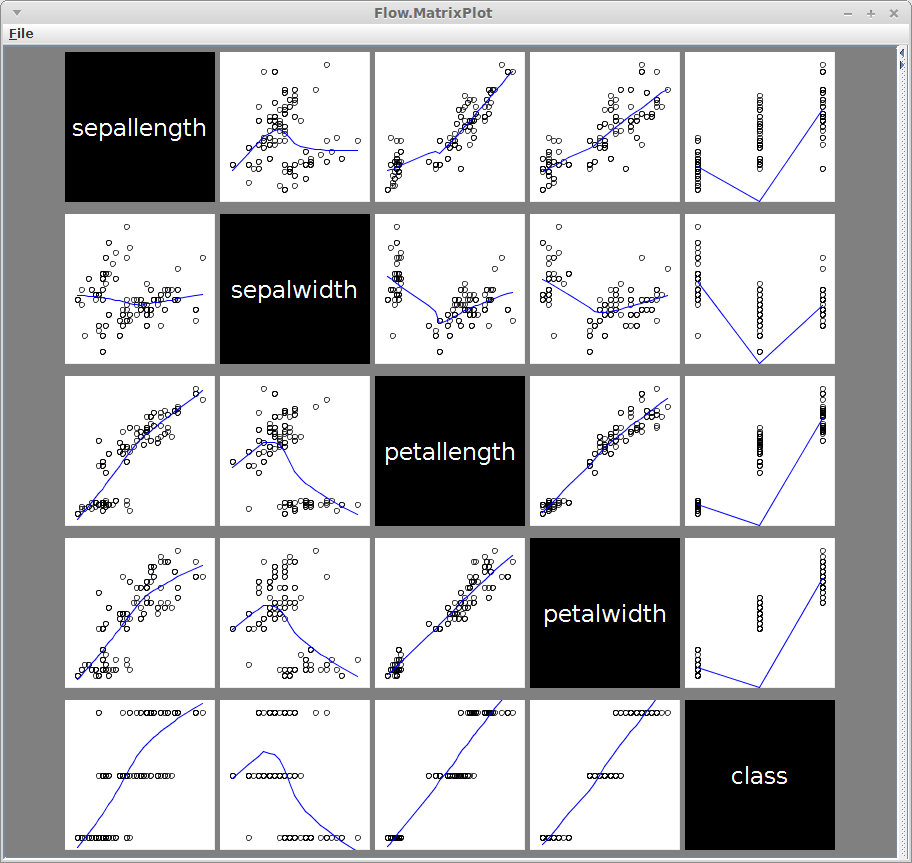
\includegraphics[width=6.0cm]{images/matrixplot-output.png}
    \caption{Matrix plot output.}
    \label{matrixplot-output}
  \end{minipage}
\end{figure}

\clearpage
\subsection{Probability plot}
The probability plot is used for visualizing predictions results, actual vs 
predicted. The plot allows you to choose from the following distributions:
\begin{tight_itemize}
	\item exponential
	\item gamma
	\item logistic
	\item $log$(logistic)
	\item normal \textit{(default)} \cite{normalprobplot}
	\item $log$(normal)
\end{tight_itemize}
Depending on the distribution, it is also possible to display a regression line,
i.e., the optimal line for predicted vs actual.

The flow\footnote{adams-visualstats-probabilityplot-slug\_ln.flow} depicted
in Figure \ref{probabilityplot-flow} uses the $log$-transformed \textit{slug} data 
(see \cite{slug}) to cross-validate LinearRegression and then displays the
predictions using the \textit{normal} distribution (see Figure \ref{probabilityplot-output}).

\begin{figure}[ht]
  \begin{minipage}[t]{0.5\linewidth}
    \centering
    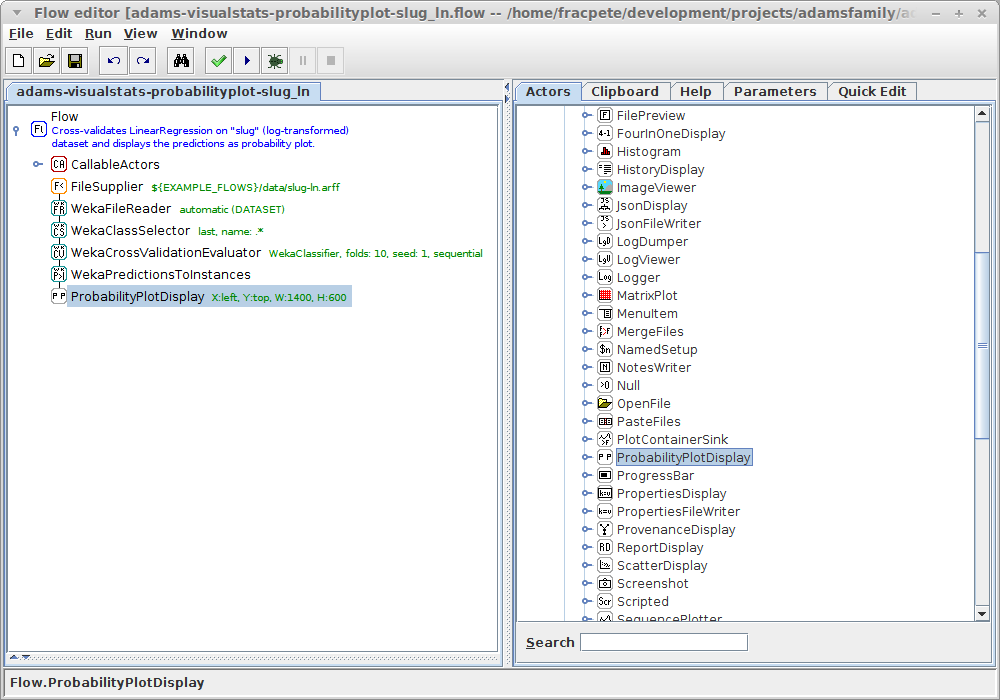
\includegraphics[width=5.5cm]{images/probabilityplot-flow.png}
    \caption{Probability plot flow.}
    \label{probabilityplot-flow}
  \end{minipage}
  \hspace{0.5cm}
  \begin{minipage}[t]{0.5\linewidth}
    \centering
    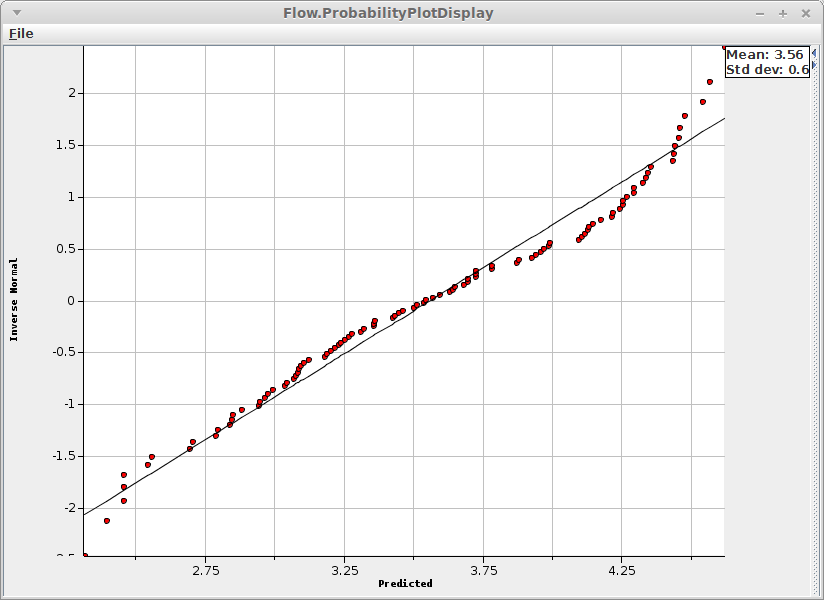
\includegraphics[width=6.0cm]{images/probabilityplot-output.png}
    \caption{Probability plot output.}
    \label{probabilityplot-output}
  \end{minipage}
\end{figure}

\clearpage
\subsection{Scatter display}
The scatter display or scatter plot allows you to plot two attributes from a 
dataset against each, one on the x-axis, the other on the y-axis. You can add
overlays to the graph, like a simple diagonal (for regression predictions this is the 
optimum when plotting actual vs predicted) or the LOWESS (locally weighted 
scatterplot smoothing). The flow\footnote{adams-visualstats-scatterdisplay-slug\_ln.flow}
shown in Figure \ref{scatterdisplay-flow} generates the output in Figure 
\ref{scatterdisplay-output}.

\begin{figure}[ht]
  \begin{minipage}[t]{0.5\linewidth}
    \centering
    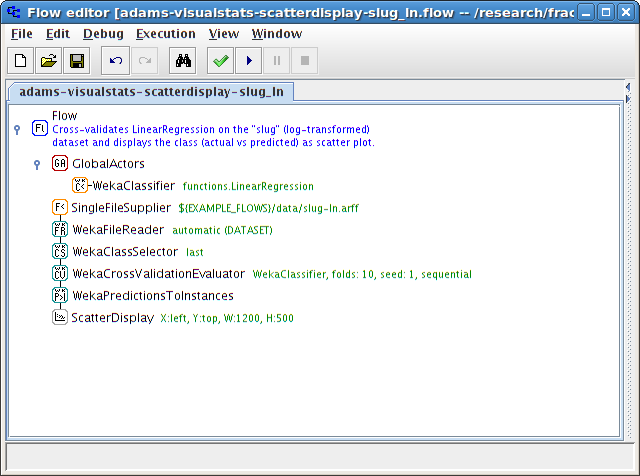
\includegraphics[width=5.5cm]{images/scatterdisplay-flow.png}
    \caption{Scatter display flow.}
    \label{scatterdisplay-flow}
  \end{minipage}
  \hspace{0.5cm}
  \begin{minipage}[t]{0.5\linewidth}
    \centering
    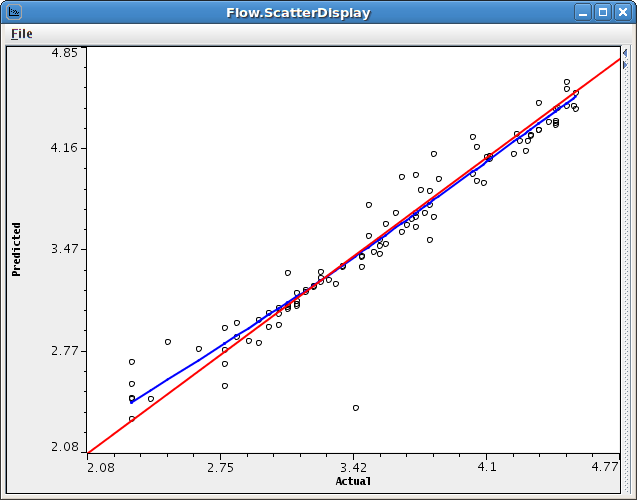
\includegraphics[width=6.0cm]{images/scatterdisplay-output.png}
    \caption{Scatter display output.}
    \label{scatterdisplay-output}
  \end{minipage}
\end{figure}

\clearpage
\subsection{Z-Score display}
The z-score (or standard score) shows how many standard deviations an
observation is off the mean. By default, the display shows markers for the mean,
at $\pm 2 \sigma$ (covers roughly 95\% of predictions) and $\pm 3 \sigma$
(covers almost all predictions). Figure \ref{zscore-flow} shows a
flow\footnote{adams-visualstats-zscore\_plot.flow} for displaying z-scores and
classifier errors. The z-score display is shown in \ref{zscore-output1} and the
classifier errors in \ref{zscore-output2}.

\begin{figure}[htb]
  \centering
  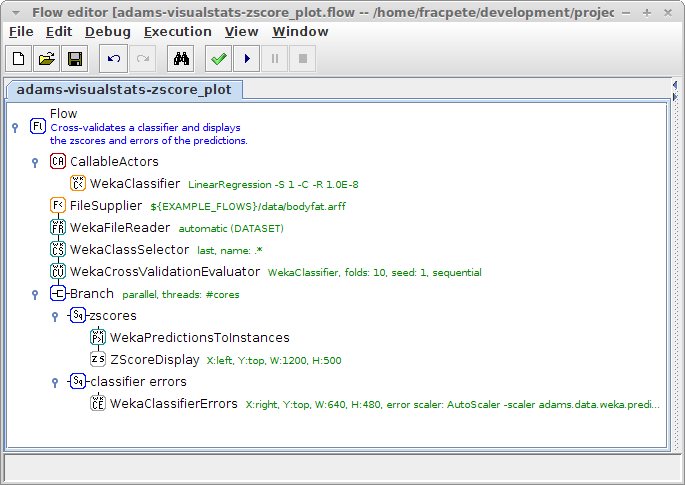
\includegraphics[width=6.0cm]{images/zscore-flow.png}
  \caption{Flow for generating z-scores.}
  \label{zscore-flow}
\end{figure}

\begin{figure}[ht]
  \begin{minipage}[t]{0.5\linewidth}
    \centering
    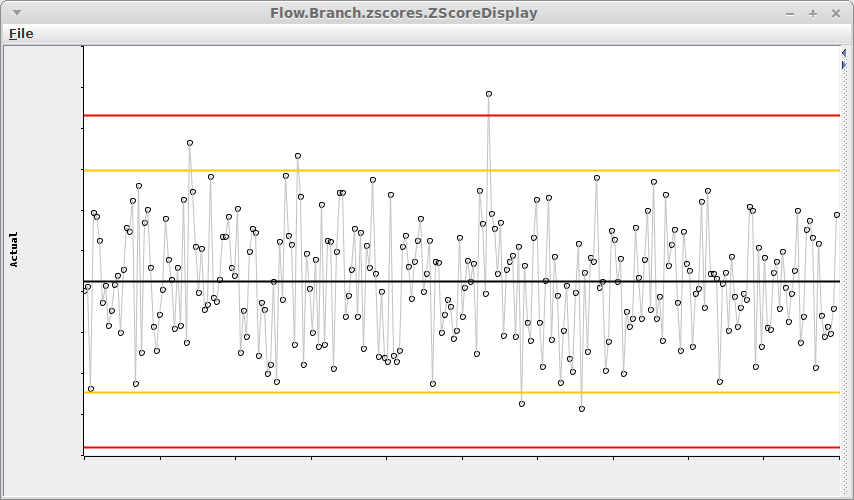
\includegraphics[width=5.5cm]{images/zscore-output1.png}
    \caption{Z-Score output.}
    \label{zscore-output1}
  \end{minipage}
  \hspace{0.5cm}
  \begin{minipage}[t]{0.5\linewidth}
    \centering
    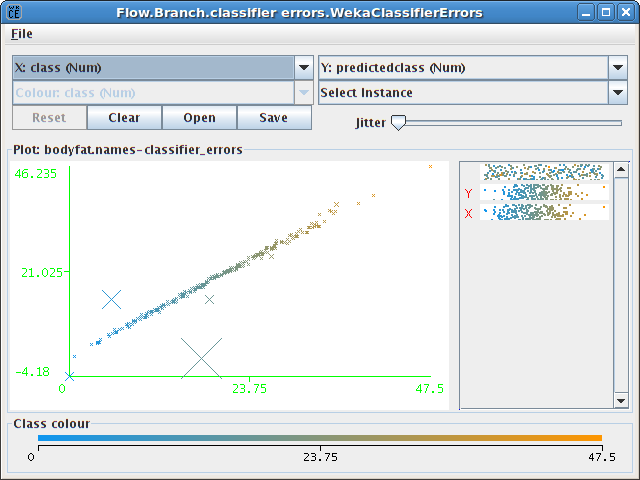
\includegraphics[width=6.0cm]{images/zscore-output2.png}
    \caption{Classifier errors output.}
    \label{zscore-output2}
  \end{minipage}
\end{figure}

%%%%%%%%%%%%%%%%%%%%%%%%%%%%%%%%%%%
% Copyright (c) 2009-2012 by the University of Waikato, Hamilton, NZ. 
% This work is made available under the terms of the 
% Creative Commons Attribution-ShareAlike 4.0 license,
% http://creativecommons.org/licenses/by-sa/4.0/.
%
% Version: $Revision$

\begin{thebibliography}{999}
	% to make the bibliography appear in the TOC
	\addcontentsline{toc}{chapter}{Bibliography}

    % references
	\bibitem{adams}
		\textit{ADAMS} -- Advanced Data mining and Machine learning System \\
		\url{https://adams.cms.waikato.ac.nz/}{}

	\bibitem{esrigrid}
	 	\textit{Esri Grid} -- a raster GIS file format deveoped by Esri. \\
		\url{https://en.wikipedia.org/wiki/Esri\_grid}{}

	\bibitem{kml}
	 	\textit{Keyhole Markup Language} -- an XML notation for expressing
	 	geographic annotation and visualization within Internet-based,
	 	two-dimensional maps and three-dimensional Earth browsers. \\
		\url{http://en.wikipedia.org/wiki/Keyhole\_Markup\_Language}{}

	\bibitem{postgresql}
	 	\textit{PostgreSQL} -- a powerful, open source object-relational
	 	database system. \\
		\url{http://www.postgresql.org/}{}

	\bibitem{postgis}
		\textit{PostGIS} -- a spatial database extender for PostgreSQL
		object-relational database. It adds support for geographic
		objects allowing location queries to be run in SQL.  \\
		\url{http://postgis.net/}{}

	\bibitem{srid4269}
	 	\textit{SRID 4269} -- or NAD 83 (North American Datum). \\
		\url{http://spatialreference.org/ref/epsg/4269/}{}

	\bibitem{mysql}
		\textit{MySQL} -- an open-source relational database management
		system (RDBMS) \\
		\url{http://www.mysql.com/}{}

\end{thebibliography}


\end{document}
